
\chapter{Suchen}
Viele Arten von Suchen:
\begin{itemize}
    \item \textbf{Schlüsselsuche}: suche Elemente, deren Schlüssel einem vorgegebenen Schlüssel entspricht
    \item Bereichssuche: ein Intervall von gültigen Werten wird gesucht
    \item Nachbarschaftssuche / Ähnlichkeitssuche: Elemente, die einem gegebenen Element ähnlich sind (z.B. Internetsuche)
    \item $\underline{\text{Graphensuche}}$: suche einen Weg von einem gegebenen Knoten zu einem anderen (z.B. Navigationsprogramm)
\end{itemize}

\section{Schlüsselsuche}

\subsection*{naive Methode: sequentielle Suche}
Vorbedingungen:
\begin{itemize}
    \item Daten liegen in einem Array
    \item Datenelemente können auf Identität (==) des Schlüssels verglichen werden
\end{itemize}

\begin{minted}{python}
def sequential_search(a, target_key, key_func):
    for i in range(len(a)):
        if key_func(a[i]) == target_key:
            return i        # gefunden bei Index i
    return None             # nichts gefunden
                            # oder "return -1"
    \end{minted}

    Vereinfachung: die Datenelemente sind der Schlüssel

    \begin{minted}{python}
def sequential_search(a, target_key):   #Komplexitaet:
    for i in range(len(a)):             #O(N)
        if a[i] == target_key:          #O(1)
            return i
    return None                         #O(1)
        \end{minted}
        \begin{itemize}
            \item Fall 1: nichts gefunden: $\bigO{}(N) * \bigO{}(1) + \bigO{}(1) = \bigO{}(N)$
            \item Fall 2: gefunden: im Schnitt: $\frac{N}{2}$ Schritte $\Rightarrow \bigO{}(N)$
        \end{itemize}
        $\Rightarrow$ \glqq lineare Suche\grqq

        \subsection*{Schnellere Suche: binäre Suche}
        Vorbedingungen:
        \begin{itemize}
            \item Elemente sind in sortiertem Array
            \item auf den Elementen gibt es eine totale Ordnung \\
            $\Rightarrow$ impliziert Identität: a==b $\Leftrightarrow$ not(a$<$b) and not (b$<$a)
        \end{itemize}

        $\Rightarrow$ Suche nach devide-and-conquer Prinzip\\
        \begin{minted}{python}

 a = [...]
 a.sort()
 found = binary_search(a, target_key)

 def binary_search(a, target_key):
     return binary_search_impl(a, target_key, O, len(a))

 def binary_search_impl(a, target_key, start, end):
     size = end - start
     if size <= 0:
         return None                    # nichts gefunden
     center = (start+end) // 2          # floor-Division
     if a[center] == target_key:
         return center                  # gefunden bei Index center
     elif a[center] < target_key:
         return binary_search_impl(a, target_key, center+1, end)
     else:
         return binary_search_impl(a, target_key, start, center)
        \end{minted}

        \subsection*{Komplexität der binären Suche}

        \begin{itemize}
            \item vorab: Sortieren O(N log N)
            \item Alg. selbst: V(N) = 2 + V(N/2) = 2 + 2 + V(N/4) = ...\\
            \hspace*{3cm} = $\underbrace{ 2 + 2 + ... + 2}_{[ log_2(N)] \text{Summanden}} = 2* \lceil log_2 (N) \rceil = O(logN)$
        \end{itemize}
        \begin{itemize}[label={$\Rightarrow$}]
            \item wesentlich schneller als sequentielle Suche, \textbf{aber} man muss vorab sortieren
            \item Sortieraufwand amortisiert sich über viele Suchanfragen, wenn man mindestens $\Omega(log N)$ Suchen ausführt
        \end{itemize}

        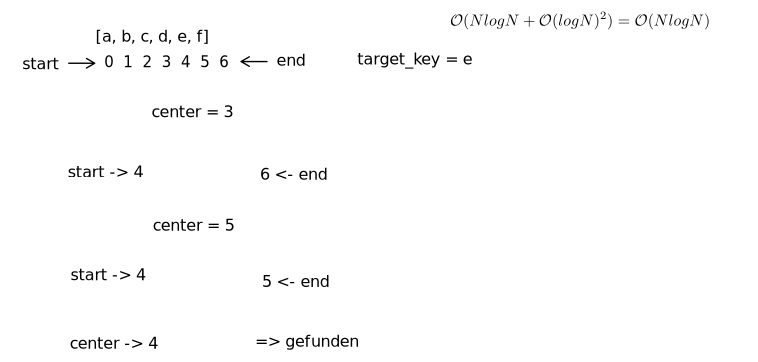
\includegraphics[width=12cm,height=9cm,keepaspectratio]{./Pictures/binaereSuche.png}

        Anwendung: Daten werden vorab gesammelt und ändern sich dann nicht mehr\\
        $\Rightarrow$ einmal sortieren, viele Suchvorgänge\\

        ungünstig: Datenarray ändert sich häufig (Einfügen oder Löschen von Elementen)\\
        $\Rightarrow$ Sortieraufwand amortisiert sich nicht $\Rightarrow$ Suchbäume oder Hashtabelle verwenden

        \section{Suchbäume}

        \begin{itemize}
            \item effiziente Suche, wenn der Datenbestand sich häufig ändert
            \item \glqq Bäume mit Wurzel\grqq = rooted trees \\
            \begin{itemize}
                \item spezielle Graphen, wo es von jedem Knoten zu jedem anderen genau einen Weg gibt
                \item ein ausgezeichneter Knoten heißt \glqq Wurzel\grqq , die zeichnet man oben :-)\\
                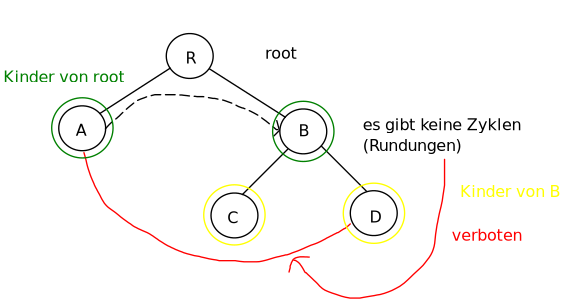
\includegraphics[width=9cm,height=7cm,keepaspectratio]{./Pictures/binaerBaum.png}
                \item speziell: Binärbäume – jeder Knoten hat maximal zwei Kinder
                \item Kinder sind Nachbarknoten, die weiter von der Wurzel entfernt sind
            \end{itemize}
            in Python: Hilfsklasse für Knoten, die ein Datenelement und maximal 2 Kinder speichert

\begin{minted}{python}
class Node:
    def __init__(self, key):
        self.key = key
        self.left = self.right = None       #anfangs keine Kinder
root = Node("R")
root.left = Node("H"); root.right = Node("B"); root.right.left = Node("C")
\end{minted}
        \end{itemize}

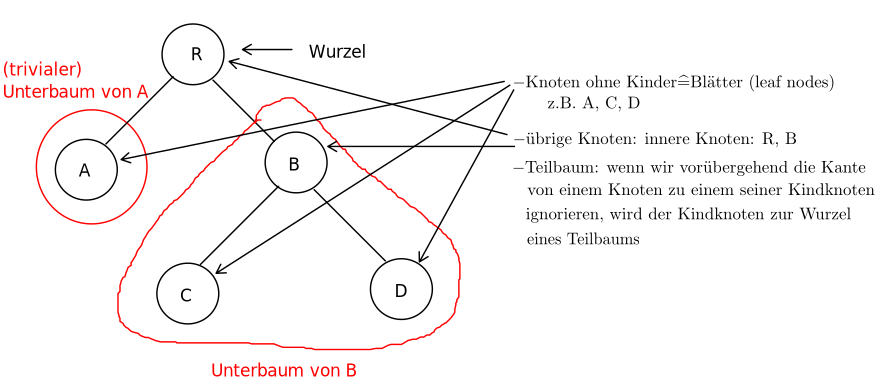
\includegraphics[width=13cm,height=10cm,keepaspectratio]{./Pictures/binaerBaum2.png}

\textbf{Suchbaum}:
\begin{enumerate}
    \item auf den Schlüsseln ist eine Ordnung definiert \glqq $<$\grqq (wie Sortieren)
    \item für jeden Knoten gilt:
    \begin{enumerate}[label=\alph*)]
        \item die Schlüssel im linken Teilbaum sind alle kleiner als der Schlüssel des Knotens
        \item die Schlüsse im rechten Teilbaum sind alle größer als der Schlüssel des Knotens
    \end{enumerate}
    (vgl.: analoges Verhalten beim Pivot in quick sort)
\end{enumerate}
\begin{itemize}
    \item zur Erinnerung: \\
    \begin{minted}{python}
class Node:
    def __init__(self, key):    #bei echten Anw: , data)
        self.key = key
        self.left = self.right = None
    \end{minted}
    \item Idee der Suche:
    \begin{itemize}
        \item wenn der Schlüssel gefunden: gib den betreffenden Node zurück
        \item sonst suche im linken oder rechten Teilbaum weiter $\Rightarrow$ \glqq teile und herrsche\grqq
        \item wenn ein Blatt und key nicht gefunden: gib None zurück
    \end{itemize}
\end{itemize}

\begin{minted}{python}
def tree_search(node, key):
    if node is None:                        # nichts gefunden, Rekursionsabschluss 1
        return None
    if key == node.key:                     # gefunden! Rekursionsabschluss 2
        return node
    if key < node.key:
        return tree_search(node.left, key)  # links weitersuchen
    else:
        return tree_search(node.right, key) # rechts weitersuchen
\end{minted}

Verwendung:
\begin{itemize}[label ={}]
    \item root = ...    \hspace*{1cm} \#Wurzel des Suchbaums
    \item result = tree\_search(root, key)
\end{itemize}
$[$ in einer Programmbibliothek würde man all das noch \glqq kapseln\grqq , so dass der Nutzer nur ein interface sieht, aber nicht die interne Funktionalität, z.B. Klasse Node $]$ \\

\textbf{Einen neuen Schlüssel in den Baum einfügen}
\begin{itemize}
    \item muss auch funktionieren, wenn Baum leer $\widehat{=}$ root = None
    \item muss auch funktionieren, wenn der Schlüssel schon vorhanden ist \\
    Möglichkeiten:
    \begin{itemize}
        \item Fehlermeldung (Exception)
        \item besser: nur die mit dem Schlüssel verknüpften Daten überschreiben \verb|a["Fritz Mueller"] = 1.0|
    \end{itemize}
\end{itemize}

\begin{minted}{python}
def tree_insert(node, key):                         # in der Praxis: ,data)
    if node is None:                                # richtigen Platz gefunden
        return Node(key)                            # Konstruktor
    if key == node.key:                             # Schluessel schon vorhanden
        return node                                 # in Praxis: Daten ersetzen vorher
    if key < node.key:                              # key gehoert in den linken Teilbaum
        node.left = tree_insert(node.left, key)     #Rekursion
    else:
        node.right = tree_insert(node.right, key)   #Rekursion
    return node
\end{minted}

Verwendung:
\begin{minted}{python}
root = None                     # leerer Baum
root = tree_insert(root, 4)
root = tree_insert(root, 2)
root = tree_insert(root, 3)
root = tree_insert(root, 6)
\end{minted}

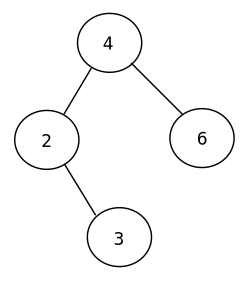
\includegraphics[width=4cm,height=4cm,keepaspectratio]{./Pictures/zahlenbaum.png}

Wenn die Schlüssel in ungünstiger Reihenfolge eingefügt werden (z.B. sortiert oder umgekehrt sortiert), erhält man statt eines Baums eine Kette ($\widehat{=}$ verkettete Liste) mit sehr langsamem Suchverhalten \\

Einfügen in der Reihenfolge 1, 2, 3, 4, 5 \\

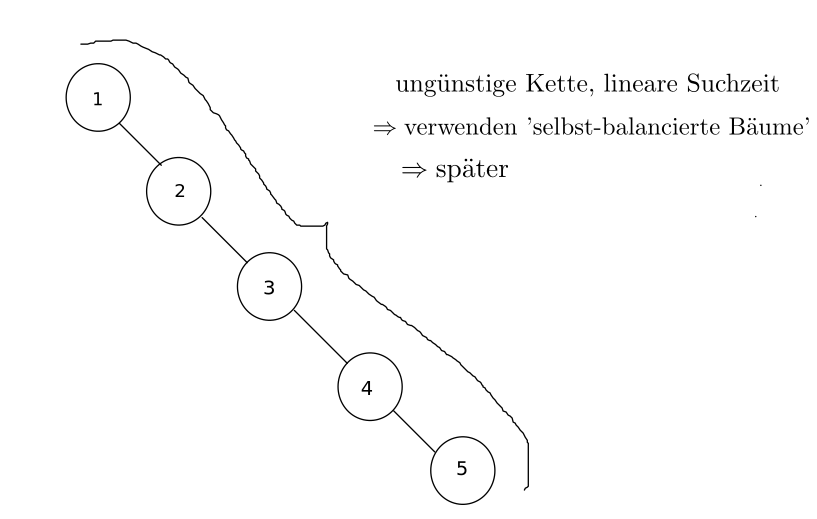
\includegraphics[width=12cm,height=7cm,keepaspectratio]{./Pictures/Kette.png}

\textbf{Entfernen eines Schlüssels aus dem Baum}\\
vier Fälle:
\begin{enumerate}
    \item der Schlüssel ist nicht vorhanden:
    \begin{itemize}
        \item Fehlermeldung
        \item remove gibt None zurück $\widehat{=}$ nichts entfernt
    \end{itemize}
    \item Schlüssel ist in einem Blatt $\Rightarrow$ kann ihn einfach entfernen
    \item Schlüsselknoten hat ein Kind $\Rightarrow$ kann ihn durch Teilbaum des Kindes ersetzen
    \item Schlüsselknoten hat zwei Kinder $\Rightarrow$ ersetze nur den Schlüssel (plus evtl. die Daten) durch den Schlüssel eines geeigneten Blatts ($\rightarrow$ der Vorgänger des zu entfernenden Schlüssels)  und entferne dann dieses Blatt
\end{enumerate}

\begin{minted}{python}
def tree_predecessor(node):
    node = node.left                # suche größten Key im linken Teilbaum
    while node.right is not None:
        node = node.right
    return node

def tree_remove(node, key):
    if node is None:  # nicht gefunden
        return None
    if key < node.key:
        node.left = tree_remove(node.left, key)
    elif key > node.key:
        node.right = tree_remove(node.right, key)
    else:  # key gefunden
        if node.left is None and node.right is None:  #Blatt
            node = None
        elif node.left is None:  # node hat nur ein Kind
            node = node.right
        elif node.right is None:  # node hat nur ein Kind
            node = node.left
        else:  # node hat 2 Kinder
            pred = tree_predecessor(node)
            node.key = pred.key  # recycle node fuer seinen Vorgaenger
            node.left = tree_remove(node.left, pred.key)
    return node
\end{minted}

Verwendung: \verb|root = tree_remove(root, key)|

%irgendwo fehlt noch die Komplexität

\subsection*{Komplexitätsanalyse der Suchbaumfunktion (ungünstiger Fall)}
zwei Möglichkeiten:
\begin{itemize}
    \item key gefunden
    \item stelle fest, dass key nicht vorhanden
\end{itemize}
intuitiv: wenn Entscheidung viele Vergleiche erfordert $\Rightarrow$ langsam \\
\textbf{Begriffe:}
\begin{itemize}
    \item \textbf{Pfade}: Folge von Knoten $n_1, n_2, \cdots, n_k$ \\
    so dass:
    \begin{itemize}
        \item $n_i$ und $n_{i-1}$ sind Nachbarn
        \item $n_1, n_n$ sind zwei Knoten, zwischen denen wir den Pfad suchen
    \end{itemize}
    \item \textbf{Länge des Pfades}: Anzahl der Kanten, k-1
    \item \textbf{Tiefe eines Knotens im Baum}: Länge des Pfades bis root
    \item \textbf{Tiefe des Baums}: maximale Tiefe eines Knotens
\end{itemize}
$\Rightarrow$ ungünstiger Fall: key wird am Ende des längsten Pfades gefunden bzw. nicht-vorhandensein festgestellt

\begin{figure}[htbp]
    \begin{minipage}[t]{6cm}
        \vspace{0pt}
        \begin{itemize}
            \item \textbf{Balance eines Baumes}: die Pfade von der Wurzel zum \glqq Entscheiden\grqq sollten möglichst ähnliche Länge haben
            \item \textbf{Trick}: zusätzlicher \emph{virtueller} Knoten $\widehat{=}$ \textbf{Sentinel}\\
            darauf zeigen alle Knoten, die den Wert None (als linkes oder rechtes Kind) speichern\\
            in Python: das None-Objekt
        \end{itemize}
        $\Rightarrow$ RS-Pfade: von root zum Sentinel
    \end{minipage}
    \begin{minipage}[t]{6cm}
        \vspace{-1cm}
        \centering
        \hspace*{2cm} 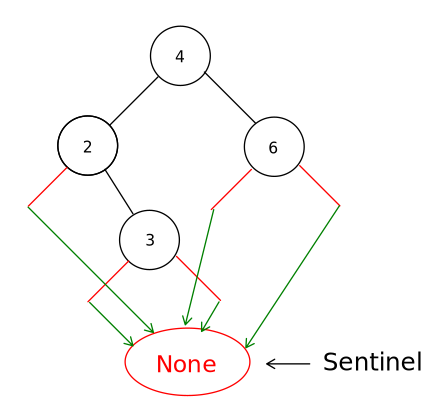
\includegraphics[width=8cm,height=8cm,keepaspectratio]{./Pictures/Sentinel.png}
    \end{minipage}
\end{figure}

\subsection{Balance des Baumes:}
Differenz zwischen kürzestem und längstem RS-Pfad

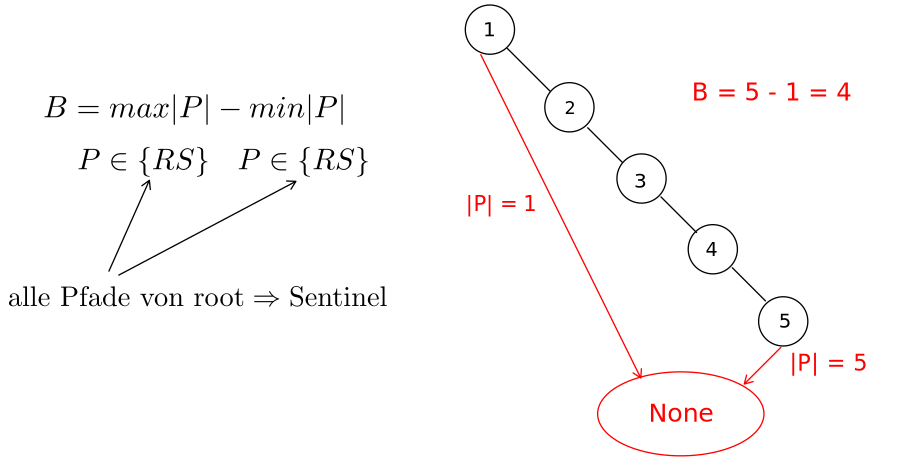
\includegraphics[width=15cm,height=5cm,keepaspectratio]{./Pictures/Kettenbalance.png}

\subsubsection{Vollständiger Baum:}
B = 0 $\rightarrow$ alle Knoten haben entweder 2 oder 0 Kinder

\begin{figure}[htbp]
    \begin{minipage}[t]{8cm}
        \vspace{0pt}
            \centering
             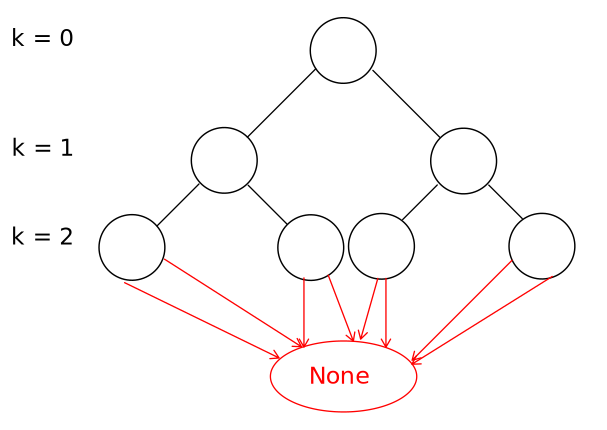
\includegraphics[width=8cm,height=4cm,keepaspectratio]{./Pictures/vollstBaum.png}
    \end{minipage}
    \begin{minipage}[t]{6cm}
        \vspace{1cm}
        Anzahl der Knoten im vollständigen Baum: bei Tiefe $k$ gibt es immer $2^k$ Blätter \\
        \hspace*{1cm} $N = 2^0 + 2^1 + \cdots + 2^{D+1} -1$ \\
        \hspace*{1cm} $D \widehat{=}$ Tiefe
    \end{minipage}
\end{figure}

\subsubsection{Perfekt balancierter Baum}
B $\leq$ 1 \\
$\Rightarrow$ für jeden Knoten gilt:
\begin{figure}[htbp]
    \begin{minipage}[t]{8cm}
        \vspace{0pt}
        \centering
        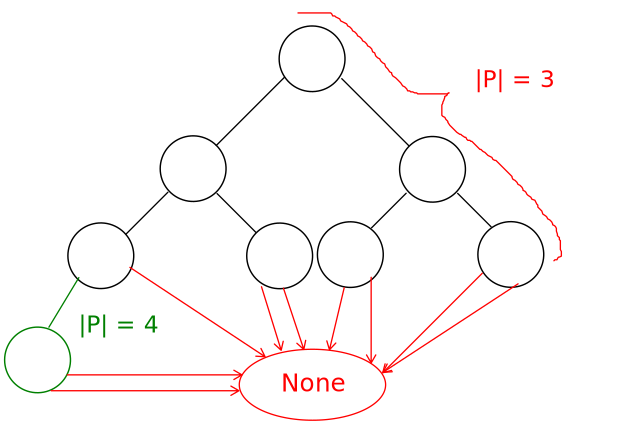
\includegraphics[width=8cm,height=5cm,keepaspectratio]{./Pictures/perfektbalanBaum.png}
    \end{minipage}
    \begin{minipage}[t]{6cm}
        \vspace{1cm}
        \begin{itemize}
            \item linker und rechter Unterbaum sind auch perfekt balanciert
            \item Tiefen von linkem und rechtem Unterbaum unterscheiden sich höchstens um 1
        \end{itemize}
    \end{minipage}
\end{figure}

\section{Balance von Suchbäumen}
B = (längster Pfad Wurzel $\rightarrow$ Sentinel) - (kürzester Pfad Wurzel $\rightarrow$ Sentinel)

\begin{figure}[htbp]
    \begin{minipage}[t]{8cm}
        \vspace{0pt}
        \centering
        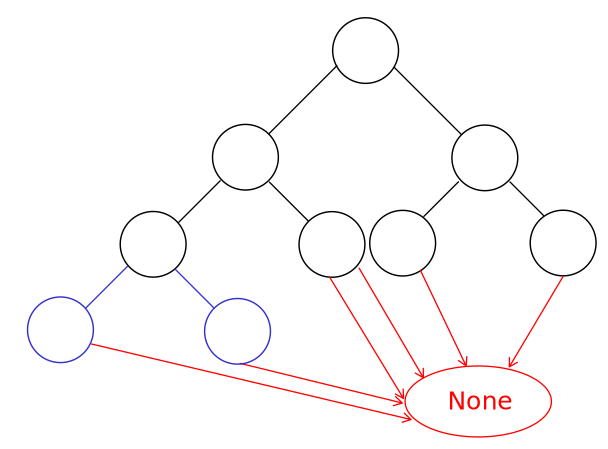
\includegraphics[width=8cm,height=5cm,keepaspectratio]{./Pictures/BalanBaum.png}
    \end{minipage}
    \begin{minipage}[t]{6cm}
        \vspace{1cm}
        \begin{itemize}
            \item vollständiger Baum, Tiefe 2
            \item \textcolor{blue}{perfekt balancierter Baum der Tiefe 3, d.h. B $\leq$ 1}
        \end{itemize}
    \end{minipage}
\end{figure}

Wieviele Elemente hat ein perfekt balancierter Baum der Tiefe $d$?
\begin{itemize}
    \item für Tiefe $d$ muss es mindestens ein Element mit Abstand $d$ von der Wurzel geben \\
    $\Rightarrow$ mindestens ein Element mehr als der vollständige Baum der Tiefe ($d$-1): $N_v = 2^d -1$\\
    $N_p \geq 2^d$
    \item um in die Tiefe $d$ zu passen, darf der perfekt balancierte Baum höchstens ein vollständiger Baum sein $\Rightarrow$ $N_p \leq 2^{d+1} -1$
\end{itemize}
\begin{itemize}[label={$\Rightarrow$}]
    \item Komplexität der Suchoperationen: Anzahl der Vergleiche $\widehat{=}$ Länge des längsten RS-Pfades im ungünstigsten Fall, \textcolor{red}{$V \in \bigO{}(d)$} beim perfekt balancierten Baum der Tiefe $d$ \\
    \[ 2^d \leq N_p \leq 2^{d+1} - 1 \hspace*{2cm} log_2(2^d) \leq log_2(N_p) \leq log_2(2^{d+1}-1) < log_2(2^{d+1})\]
    \item $d\leq log_2(N_p) < d + 1 \Rightarrow$ \textcolor{red}{$V \in \bigO{}(d) \Leftrightarrow \bigO{}(log N_p)$}\\
    \textcolor{red}{wie bei binärer Suche, also schnell.}
    \item Folgerung:
\end{itemize}wenn Baumoperationen schnell sein sollen, müssen wie sicherstellen, dass der Baum balanciert ist $\Rightarrow$ nach jedem insert oder remove wird die Balance \glqq repariert\grqq

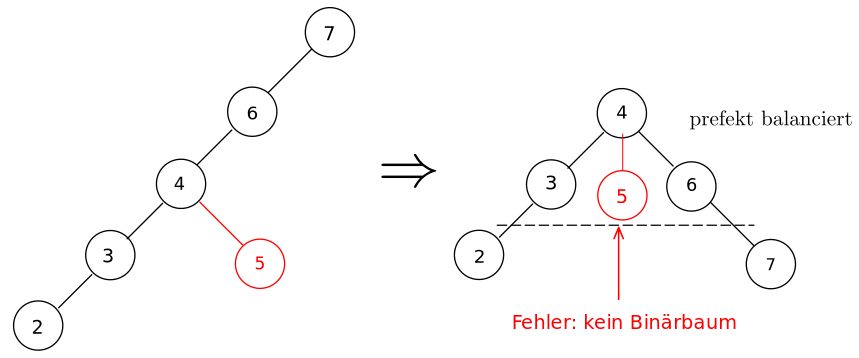
\includegraphics[width=15cm,height=5cm,keepaspectratio]{./Pictures/Reparatur.png}

3 Regeln für die Reparatur:
\begin{enumerate}
    \item Der Baum muss ein Binärbaum bleiben
    \item Die Suchbaumbedingung muss weiter gelten
    \item Die Reparatur soll lokal erfolgen (in der Nähe des aktuellen Knotens) $\Rightarrow$ Effizienz
\end{enumerate}

Grundlegende Operation: \textbf{Baumrotation}: ändert die Wurzel eines Teilbaums nach obigen Regeln, so dass Balance besser wird

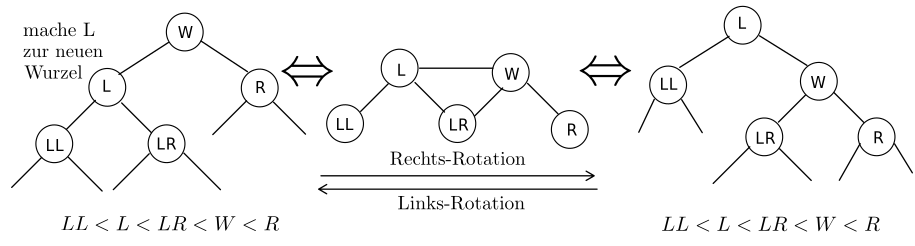
\includegraphics[width=16cm,height=6cm,keepaspectratio]{./Pictures/Rotation.png}

in Python:
\begin{minted}{python}
def tree_rotate_right(node):
    new_root = node.left
    node.left = new_root.right
    new_root.right = node
    return new_root
\end{minted}

\begin{minted}{python}
def tree_rotate_left(node):
    new_root = node.right
    node.right = new_root.left
    new_root.left = node
    return new_root
\end{minted}

Beispiel: AVL-Bäume
\begin{itemize}
    \item transformieren den Baum immer in perfekte Balance
    \item aber: das ist schwierig und unnötig,
\end{itemize}
\begin{itemize}[label={$\Rightarrow$}]
    \item \glqq einfache\grqq Balance reicht aus: \[ V \in \bigO{}(d)\]
    \[ V \leq c - d \text{ für geeignete Konstante (unabhängig von d bzw. N)}\]
    \item wenn die Tiefe nur um einen konstanten Faktor schlechter ist als beim perfekt balancierten Baum, verschwindet die Konstante in $\bigO{}(d)$ $\Rightarrow$ gleiche Komplexität
    \item viel einfachere Implementation \\
    Beispiele:
    \begin{itemize}
        \item Rot-Schwarz-Baum (typische Implementation)
        \item Treap ($\Rightarrow$ siehe Hausaufgabe)
        \item Anderson-Baum (Vereinfachung des Rot-Schwarz-Baum)
    \end{itemize}
\end{itemize}

\section{Anderson-Bäume}
Idee: jeder Knoten hat ein \emph{level} $\widehat{=}$ Abstand (kürzester Pfad) zum None-Sentinel

\begin{minted}{python}
class AndersonNode:
    def __init__(self, key):
        self.key = key
        self.left = self.right = None
        self.level = 1  #distance to None in left and right
\end{minted}

Idee: Im Anderson-Baum gibt es
\begin{itemize}
    \item horizontale Kanten (parent.level == child.level)
    \item vertikale Kanten (parent.level == child.level + 1)
\end{itemize}
\textbf{Regeln:}
\begin{itemize}
    \item die reduzierte Länge eines Pfades r: nur die vertikalen Kanten gezählt
    \item Sentinel hat level == 0 und alle Kanten zum Sentinel sind vertikal \\
    $\Rightarrow$ echte Knoten haben level $\geq$ 1
    \item reduzierte Höhe ($h_r$)  eines Knotens entspricht der reduzierten Pfadlänge ($r$)
    \item Alle RS-Pfade haben die \textbf{gleiche} reduzierte Länge. $\Rightarrow$ jeder Knoten, insbesondere die Wurzel werden auf allen Pfaden von None nach der gleichen Anzahl vertikaler Kanten erreicht (\emph{aber}: die Anzahl horizontaler Kanten kann verschieden sein)
    \item kein Pfad darf zwei horizontale Kanten hintereinander haben
    \item Vereinfachung durch Anderson: nur Kanten zum rechten Kind dürfen horizontal sein (sonst: Rot-Schwarz-Baum)
\end{itemize}
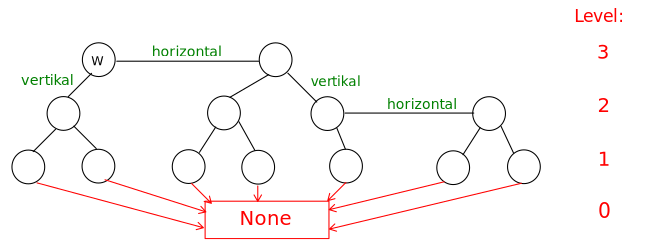
\includegraphics[width=16cm,height=4.5cm,keepaspectratio]{./Pictures/Anderson.png}

\textbf{Satz:} jeder Anderson-Baum ist balanciert (höchstens einen konstanten Faktor schlechter als der perfekt balancierte Baum), Beweis:
\begin{enumerate}
    \item $h_r$ = reduzierte Höhe des Baums (Abstand Wurzel $\rightarrow$ Sentinel \emph{ohne} horizontale Kanten)
    \begin{itemize}
        \item hat der Baum \emph{keine} horizontalen Kanten $\Rightarrow$ vollständiger Baum Tiefe $d_v = h_r - 1$
        \item hat der Baum horizontale Kanten, hat er \emph{mehr} Konten als der vollständige Baum
        \[ N \geq 2^{d_v +1} - 1 = 2^{h_r}-1\]
    \end{itemize}
    \item Da nie zwei horizontale Linien aufeinander folgen, ist die tatsächliche Tiefe höchstens zweimal die reduzierte Tiefe: $d \leq 2 * h_r$
    \item Zusammenfassen
    \[ N \geq 2^{d/2} - 1 \hspace*{2cm} N+1 \geq 2^{1/2} \]
    \[ log_2(N+1) \geq d/2 \hspace*{1.2cm} d \leq 2 log_2(N+1)) \]
\end{enumerate}
Da der schlechteste Fall des Suche: $V \in \bigO{}(d) = \bigO{}(2 log_2(N+1))$\\
\hspace*{6.45cm} $\Rightarrow \boxed{V = \bigO{}(log N)}$ \hspace*{5cm} $\square$ \\

Prinzip, den Baum balanciert zu halten bei \emph{insert}:
\begin{itemize}
    \item füge den neuen Knoten normal ein (rekursive Aufrufe von \verb|tree_insert|)
    \item prüfe, ob die Anderson-Bedingungen beim parent des neuen Knotens verletzt sind $\Rightarrow$ repariere den Unterbaum von parent
    \item auf dem Rückweg der Rekursion: prüfe und repariere auch alle Vorfahren auf dem Pfad bis zur Wurzel
\end{itemize}
in Python:
\begin{minted}{python}
def anderson_tree_insert(node, key):
    if node is None:
        return AndersonNode(key)
    if key == node.key:
        #Daten aktualisieren
        return node
    if key < node.key:
        node.left = anderson_tree_insert(node.left, key)
    else:
        node.right = anderson_tree_insert(node.right, key)
    # bis hier wie bei tree_insert()
    # ab hier Balance reparieren
    if node.left is not None and node.level == node.left.level:
        node = tree_rotate_right(node)      #turn left horizontal into right horizontal
    if node.right is not None and node.right.right is not None and node.level == node.right.right.level:    #zwei horizontal hintereinander
    # node.right -> anheben und zur Wurzel machen
    node = tree_rotate_left(node)
    node.level += 1
    return node
\end{minted}
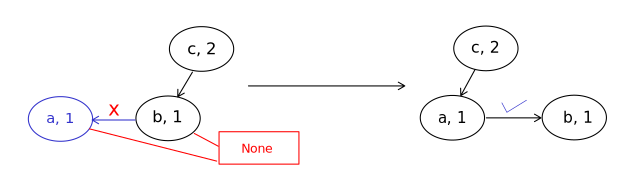
\includegraphics[width=16cm,height=3cm,keepaspectratio]{./Pictures/AndersonPython1.png}

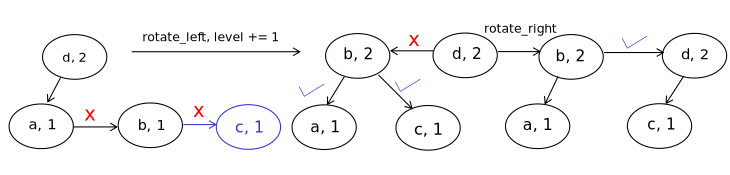
\includegraphics[width=16cm,height=3cm,keepaspectratio]{./Pictures/AndersonPython2.png}

\section{Prioritätssuche}
\begin{itemize}
    \item Variante der Suche: statt nach einem konstanten Schlüssel suchen wir den
    \begin{itemize}
        \item größten Schlüssel (max-priority search)
        \item kleinsten Schlüssel (min-priority search)
    \end{itemize}
    \item andere Interpretation als Verallgemeinerung von Stack und Queue, anschaulich: Elemente mit hoher Priorität dürfen in der Schlange vordrängeln
    \begin{itemize}
        \item Annahme: beim push in Stack oder Queue wird für das betreffende Element der Zeitstempel mitgespeichert
        \item definiere Priorität als $| now - timestamp_i| \Rightarrow$ höchste Priorität $\widehat{=}$ am längsten im Container \\
        \hspace*{1cm} $\Rightarrow$ first-come – first-served Verhalten $\widehat{=}$ Queue \\
        $\Rightarrow$ kleinste Priorität $\widehat{=}$ am kürzesten im Container $\Rightarrow \begin{rcases} \text{last-come – first-served} \\
            \text{last in - first out}\end{rcases}$ Stack
    \end{itemize}
        \item elementare Eigenschaft: max priority search $\Leftrightarrow$ zu min priority search mit negierten Schlüsseln
        \item naive Implementation: sequentielle priority search:
        \begin{minted}{python}
def sequential_priority_search(a):  #max priority
    m = 0
    for i in range(1, len(a)):
        if a[i] > a[m]:
            m = i
    return m        # Index des groessten Elements
    # => innere Schleife von selection sort (aber min priority) => O(N)
        \end{minted}
        \item Implementation mittels Suchbaum: das größte Element ist das \glqq rechteste Kind\grqq
        \begin{minted}{python}
def tree_priority_search(node):
    if node is None:
        raise KeyError("empty tree")
    while node.right is not None:
        node = node.right
    return node
    # => sehr aehnlich zu tree_predecessor (aber min pr.) => O(d) = O(log N) im balancierten Baum
        \end{minted}
        \item Beobachtung: $\bigO{}(logN)$ kann man viel einfacher erreichen als mit einem Suchbaum $\Rightarrow$ Heap (\glqq priority search tree\grqq  )
        \begin{itemize}
            \item ersetze Suchbaumbedingung durch Heapbedingung: \\
            \glqq kein Schlüssel im linken oder rechten Teilbaum hat höhere (niedrigere) Priorität als die Wurzel jedes Teilbaums im max heap (min heap)\grqq
            \item das erweist sich als viel einfacher, weil man
            \begin{enumerate}
                \item immer einen perfekt balancierten Baum garantieren kann (ohne komplexe Umstrukturierungen wie beim Andersson-Baum)
                \item den Baum als Array (= sehr effizient) speichern kann
            \end{enumerate}
        \end{itemize}
        $\Rightarrow$ linkslastigeR perfekt balancierteR Baum kann eindeutig \glqq geflattet\grqq werden, d.h. als Array \glqq flachgedrückt\grqq
        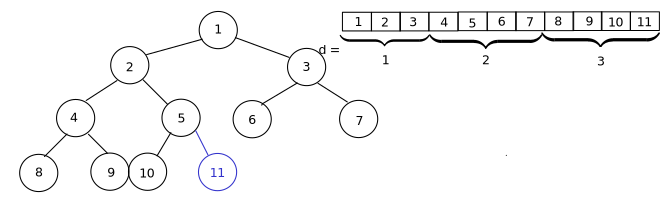
\includegraphics[width=16cm,height=4cm,keepaspectratio]{./Pictures/Flatten.png}
        \begin{itemize}
            \item Adressierung der Knoten im geflatteten Baum a \\
            \begin{itemize}
                \item a[0] $\Rightarrow$ Wurzel
                \item a[1], a[2] linkes und rechtes Kind der Wurzel
                \item a[3], a[4] linkes und rechtes Kind von a[1] usw.
                \item generell gilt:
                \begin{itemize}
                    \item die Kinder von a[i] sind a[2*i + 1] linkes Kind \\
                    \hspace*{8cm} a[2*i + 2] rechtes Kind
                    \item der Parent von a[i] ist a[(i-1) // 2] (floor division $\rightarrow$ abrunden)
                \end{itemize}
                \item die Umrechnungen ersetzen die Zugriffe \verb|node.left| und \verb|node.right| im Suchbaum
            \end{itemize}
        \end{itemize}
        \item aus der Heap-Bedingung folgt: das Element mit größter Priorität ist immer die Wurzel des ganzen Baums: a[0]
        \begin{minted}{python}
def heap_largest(a):
    return a[0]         #Komplexitaet O(1)
        \end{minted}
        \item Einfügen in den Heap: Nutze die Eigenschaft des dynamischen Arrays, das Einfügen am Ende billig ist (amortisiertes $\bigO{}(1))$:
        \begin{itemize}
            \item füge neue Elemente am Ende an (dann bleibt der Baum linkslastig perfekt balanciert)
            \item repariere eventuell die Heap-Bedingung, falls das neue Element größer als sein parent ist.
        \end{itemize}
        in Python:
        \begin{minted}{python}
def heap_insert(a, key):        #max heap
    a.append(key)               #am Ende anhaengen
    upheap(a, len(a)-1)     #reparieren des aktuell gueltigen Bereichs

def upheap(a, k):
    v = a[k]        #zwischenspeichern
    while True:     #Endlosschleife (durch "break" verlassen)
        if k == 0:  #a[k] Wurzel
            break   #Heap-Bedingung auf jeden Fall erfuellt
        parent = (k-1) // 2
        if a[parent] > v:   #Heap-Bedingung erfuellt
            break
        a[k] = a[parent]    #Heap-Bed. reparieren: parent eine Ebene nach unten schieben
        k = parent
    a[k] = v    #Element v korrekt einsortieren
        \end{minted}
        Komplexität
        \begin{itemize}[label={}]
            \item $\widehat{=}$ Anzahl der Durchläufe durch while-Schleife
            \item $\leq$ der ursprünglichen Tiefe des Knotens $ k \in \bigO{}(logN)$
        \end{itemize}
        \item analog funktioniert das Entfernen: \verb|pop()| $\Leftrightarrow$ \verb|remove_largest()| \\
        Idee:
        \begin{itemize}
            \item tausche Wurzel mit dem letzten Element des Arrays
            \item Entferne letztes Element (amortisiert $\bigO{}(1)$)
            \item repariere die Heap-Bedingung, wenn neue Wurzel nicht größtes Element
        \end{itemize}
        \begin{minted}{python}
def heap_remove_largest(a):
    a[0] = a[len(a) - 1]        #largest ersetzen
    del a[len(a) - 1]           #letztes loeschen
    # = a[-1]
    downheap(a)             #Heap-Bedingung reparieren

def downheap(a, last = None):
    if last is None: last = len(a) - 1
    k = 0   #Wurzel ist eventuell nicht das groesste Element
    v = a[k]
    while True:     #ab hier insgesamt: O(d) = O(log N)
        child = 2 * k + 1   #Index des linken Kinds
        if child > last:    #Kind existiert nicht => Heap-Bedingung erfuellt
            break
        if child + 1 <= last and a[child] < a[child + 1]:
        # rechtes Kind existiert & rechtes Kind hat hoehere Prioritaet als linkes
            child = child + 1
        if v >= a[child]:   #Heap-Bedinung erfuellt
            break
        a[k] = a[child]     #child eine Ebene hoch
        k = child
    a[k] = v                # Element v korrekt einsortieren
        \end{minted}
        \item aus dem Heap-Verhalten kann man einen effizienten Sortieralgorithmus ableiten:
        \begin{itemize}
            \item Idee: unsortiert in den Heap einfügen, immer das größte wieder entnehmen\\
            $\Rightarrow$ man bekommt die Elemente in absteigender Sortierung
            \item Komplexität: $\bigO{}(N log N)$ wie Merge sort
            \item überraschende Beobachtung: das geht in-place: man braucht nur das Array für den geflatteten Heap, wie Quick Sort
            \item in Python:
            \begin{minted}{python}
a = ... # unsortiertes Array, benutze gleichzeitig als Heap
heap_sort(a)
def heap_sort(a):
    N = len(a)
    for k in range(1, N):  #Einfuegephase
        upheap(a, k)
    # jetzt ist a ein Heap, d.h. so sortiert, dass die Heap-Bedingung gilt
    for k in range(N - 1, 0, -1):  # Entfernungsphase
        #groesstes Element an die sortierte Position bringen
        a[0], a[k] = a[k], a[0]
        downheap(a, k - 1)  #repariere Heap bis Indes k - 1 ("Restheap")
            \end{minted}
        \end{itemize}
\end{itemize}

